% document de test for report-DMKM.cls (LaTeX2e)
% Created May 15, 2012

% We use the style given in rapport-DMKM.cls
\documentclass{report-DMKM}

% this package (optionnal) allows merging rows and columns in latex table 

\usepackage{multirow}

%The following fields (title, author, date, tutors et place) must be present
\title{Mining parliamentary data and news articles \newline to find patterns of collaboration between politicians and third party actors}
\author{Francisco Andr\'es RODR\'IGUEZ DRUMOND}
% Defense date
\date{July 7th, 2014}
\tutors{\mbox{Marta Arias, Universitat Polit\`ecnica de Catalunya},\newline
        Josep Larriba, Data Management group (DAMA-UPC),\newline}

\place{Data Management group, Barcelona, Spain.}
% You can add the logo of the institution where you carry out your internship. Example here ERIC lab

\logo{img/dama_logo.jpg}{25mm} 

\begin{document}

% Cover page (mandatory)
\maketitle

\newpage
% summary in English  (mandatory)
\begin{abstract}
LOPEN IPSUM
\end{abstract}

% summary in French  (mandatory)
\begin{resume}
LOPEN IPSUM
\end{resume}

% table of content   (mandatory)
\tabledesmatieres

\section*{Hosting institution}

This Master's thesis was done with the support and supervision of the DAMA and LARCA Research Groups at Universitat Polit\`ecnica de Catalunya (UPC). 

\subsection*{DAta MAnagement group - DAMA}

DAMA-UPC is part of the Computer Architecture Department (DAC). The main research topics of DAMA-UPC are oriented to performance, exploration and quality in data management, focusing particularly on large data volumes. Specifically, they have investigated the creation of new data structures, algorithms, methods and applications in the area of Data Management that make it easier to manipulate large amounts of data.\\

DAMA-UPC is a member of Tecnio since 2005. Tecnio is an initiative of ACC10, the Agency for Innovation and Internationalization of the Catalan Enterprise, belonging to Generalitat de Catalunya. It is supported by Generalitat de Catalunya as a Consolidated Research Group (SGR-1187) and by the Ministry of Education and Science of Spain. Since its creation it has worked with important technological partners such as IBM, Oracle technologies, the Ministry of Cience and Innovation, the Health Department of the Generalitat de Catalunya, among others; and is current participating in four European Research Projects. \\

Moreover, DAMA-UPC has been a pioneer in scientific collaboration, creating and organizing for three consecutive years the Workshop on Graph-based Technologies and Applications (Graph-TA), organizing the 17th International Database Engineering \& Applications Symposium (IDEAS 2013) and the First University-Industry Meeting on Graph Databases (UIM-GDB). The work of DAMA has also give birth to Sparksee, a graph database, and Sparsity Technologies.\\

\subsection*{Laboratory of Relational Algorithmics, Complexity and Learnability - LARCA}

LARCA is an international research group working on data mining, machine learning, data analysis, and mathematical linguistics. They typically approach problems from sound mathematical principles, using modelling tools and techniques from algorithmics, computational complexity, automata theory, logic, discrete mathematics, statistics, and dynamic systems. \\

LARCA has also participated in several European research projects and collaborated with several industrial partners including Gas Natural Fenosa, Xopie, 4dLife, Urbiotica and Vingenia. They also foster collaboration with other research groups in and outside of Spain, including ALBCOM: Algorithms, Computational Biology, Complexity and Formal Methods Research Group at CS-UPC; NLP: Natural Language Processing Research Group at CS-UPC; IAIA: Investigacion y Aplicaciones en Inteligencia Artificial group at U. M\'alaga; CCG: Computational Complexity Group at U. Zaragoza; MIDAS: Spanish Network on Data Mining and Learning; Machine Learning Group at the University of Waikato, New Zealand and the Real and functional Analysis Research Group of Universitat de Barcelona. \footnote{Text partially taken from \url{www.dama.upc.edu} and \url{https://recerca.upc.edu/larca/}}

\newpage
\section{Acknowledgement}

LOREM IPSUM

\newpage
\section{Introduction}\label{sec:intro}

Modern law-making is characterized by the indirect participation of third-parties in the legislative process to attempt to influence the contents and outcome of the discussions according to their interests. This process, known as \emph{lobbying}, is regularly done by companies, Non-Governmental Organizations (NGOs) and in some cases citizens and foreign governments. For instance, when a law concerning human rights is being discussed in a parliament we can expect human rights NGOs to contact politicians to attempt to push their agenda. \\

Most of the times citizens are completely unaware of the lobbying activities of their representatives. This is due to the fact that it is hard to closely monitor the activities of politicians, to understand the intricacies behind the drafting of bills and to grasp the implications they have on organizations and society. Knowing how decisions makers are influenced is however of great interest for politologists, journalists and voters in general. By tracking these relations we would be able to understand better the way decisions are made by government, have a better sense of who politicians are, who they serve and what their agenda is, and in some cases fight corruption. \\

\emph{Policy Network Analysis} (PNA) is the discipline in Political Science which is focused on the discovery and analysis of links between government and other members of a society, with a particular interest in the understanding of the policy making process and its outcomes. There are plenty of definitions of Policy Networks (PN) in the literature, basically because there are many ways to characterize relationships between actors of a society and several ways to approach the analysis. However the Oxford Handbook of Public Policy proposed a definition which is widely accepted and encompasses many of the other proposals. They state that a PN is a ``set of formal institutional and informal linkages between governmental and other actors structured around shared if endlessly negotiated beliefs and interests in public policy making and implementation''\cite{moran2008oxford}. \\

One of the main difficulties in PNA is that the generation of these PN is usually done in manual, cumbersome processes by experts. This involves the use of interviews, questionnaires and other instruments from the social sciences. During the actual generation of the network many subjective factors may come into play as the overall result depends on the people involved in the study. Consequently, PN generation involves a significant investment that does not always ``lead to breathe taking empirical and theoretical results'' \cite{kenis1991policy}. The question is consequently, how can we use technology to improve the process of PN identification. \\

In this study we are concerned with the automatic generation of PN surrounding the Legislative Branch of government. The Legislative Branch is particularly interesting in the context of lobbying and policy making analysis as it is the branch of government devoted to the writing and passing of laws and regulations; the ratification of international treaties and the oversight of other branches of government. This makes parliaments particularly influential in the shaping of a society and its institutions.\\ 

Recently, there has been considerable work in the development of data mining tools for understanding the way legislative bodies work. Social Network Analysis (SNA) has been widely used to understand the dynamics of complex social systems and is a natural tool for modelling the dynamics of power in a parliament. There is a wealth of knowledge to be extracted from parliamentary data to model relationships between politicians, identify key players and sub-communities, predict the voting of bills and in general gain a better understanding of the legislative process. However, finding political relations between representatives and third party actors, who often do not appear in bills or in the transcripts of debates, remains a challenge. \\

News articles on the other hand contain a sizable amount of information about what happens in a given country and about its relevant actors. Because of this, there is plenty of work by the scientific community to develop methods to automatically extract useful knowledge from news articles. The development of applications to automatically generate Social Networks (SN) from corpora of news articles is particularly interesting in our context. This has been done extensively in the past in different areas including defense, counter-terrorism, news summarization and crime prevention. The working assumption is that by detecting patterns of co-occurrence of two entities in text we can establish that they are in some way related.  \\

In this study we use that assumption and formulate the hypothesis that by analyzing and combining parliamentary data and news articles we can generate PN for the members of a Legislative Body. Our purpose is consequently to propose a method to automatically detect links descriptive of the political closeness of politicians and relevant actors of a country, or in other words, patterns indicative of a possible lobbying activity. To do this, we automatically analyze news articles, text of bills discussed in a parliament and the transcripts of the debates. We show that it is possible to i) track the participation and the position of a politician with respect to a law and ii) find entities in news articles which could be directly related to the contents of a law. Laws thus can then be used as a cornerstone for detecting relationships between politicians and third-party actors. These relationships can then be used to build a PN which can be analysed using SNA tools. In this document we present our proposal and show the results obtained by its application in the context of the Parliament of Catalonia. \\

It is important to clarify that despite being motivated by the detection of patterns that can be suggestive of a lobbying process, in practice we aim to find relationships of political similarity or dissimilarity between two entities. The relations found by our method do not necessarily imply that the two actors are in direct liaison;  to do so we would need to closely monitor all the activities of politicians and organizations to verify with whom they are in contact. This is naturally unreasonable due to privacy considerations. \\

We aim to detect links between entities that indicate that they are both related to a particular political decision - in our case bills -, from which we could then establish political affinity or aversion. Naturally, if two entities have highly similar political views in a broad set of issues then one can believe that they could be collaborating. This could be verified by investigative journalists and by considering other sources of information like donations information, speeches, etcetera. Regardless of the verification of a lobbying process, our method is intended to be an unbiased, low-cost, semiautomated toal to aid the process of Policy Network generation and analysis. 

The rest of this document is organized as follows: in chapter \ref{sec:related-works} we present the state of the art in the automatic generation of SN from corpora of text and in the use of SNA in the context of political science. In chapter\ref{sec:proposal} we present our proposal and in chapter \ref{sec:implementation} we present some implementation considerations deemed relevant. Next, we present the obtained results in section \ref{sec:results} along with some interesting applications of our method. Finally, we present in chapter \ref{sec:conclusions} the conclusions of our work along with some suggestions for further work.


\newpage
\section{Related works}\label{sec:related-works}

There is an increasing interest in the development of applications to generate Social Networks (SN) relating entities occurring in corpora of text. This is due to the fact that there is a growing wealth of knowledge contained in text documents which is difficult to exploit due to their unstructured nature. By generating graphs that subsume the information contained in these documents, we produce a structured view which can be analyzed using Social Network Analysis (SNA) tools. \\

In this section we present the state of the art in the generation of SN from corpora of text and some related applications that use SNA for political analysis. First in section \ref{co-occurrence} we present the entity co-occurrence approach, a simple technique that has been widely used with good results. We then show in \ref{link-characterization} relevant work by the scientific community to characterize the link between two entities in a way that can be used by SNA. We also describe in \ref{topics} methods that can be used to relate entities that despite not being mentioned in the same document might be linked by means of the broader context provided by the whole corpus of documents. Next, we present in section \ref{sna-politics} studies that use SNA for political analysis and that are related to our project. Finally, we succinctly present in \ref{framing} some considerations about how the state of the art was taken into account when making our proposal.\\

\subsection{Entity co-occurrence: a first step towards the creation of SN}\label{co-occurrence}

One of the most widely used approaches to generate SN from text consists in relating entities based on their co-occurrence in a certain context. The underlying assumption of this approach is that if two entities are consistently mentioned together then they are probably related. There are several variants depending on the granularity of the context; one can look for co-occurrence within a certain sentence, paragraph, document or cluster of documents. The choice depends on the amount of data available - finer granularity probably requires more documents to produce more relations - and on the application. \\

The authors of \cite{narcho-networks} propose a method to automatically generate a social network of narco-traffickers in Mexico based on the co-occurrence of names in books about the topic. They do Entity Recognition (ER) to produce a list of entities which is then manually curated and used to determine links between drug dealers. The weight of the relationship is the count of repetitions of the co-occurrences of two entities within a certain distance. They use different network analysis tools to show how the obtained graph closely resembles the different cartels and their chain of command. \\

Similarly, the Joint Research Centre of the European Commission has done extensive work in extracting entities and inter-entities relations from newspapers written in different countries of the European Union. In \cite{jrc-main} we find a summary of their work, which is explained in depth in \cite{jrc-2} and \cite{jrc-3}. Essentially, they look for co-occurrence of entities within previously built clusters of articles that represent a story. They take into account entity coreference and use different heuristics to improve the entity recognition and disambiguation processes. They also produced a formula to measure the strength of a link based not only on the number of co-occurrences but also the frequency of the entities in the clusters and the corpus. By doing this, they aim to weight down relationships in which one of the entities is frequently mentioned, so that only relevant relationships are chosen. \\

Another interesting aspect of their proposal is the use of Wikipedia for validating the obtained graphs. Because we are in presence of a knowledge discovery task for which we do not have a ground truth set, it is difficult to evaluate if the detected links between two entities are meaningful. The definition of a meaningful link is itself not an easy task. The authors of the Joint Research Centre look for the Wikipedia pages of the detected entities and verify if there are links between pages that correspond to the links detected by the system. They define a ``strong'' relationship as one in which there is a reciprocal presence of a link.This allows for the creation of a ground truth set which can be used to evaluate the system with the standard precision and recall metrics. \\

On a different note, the authors of  \cite{google-similarity-measure} present a technique to measure the semantic similarity of two words or phrases by using the Google search engine. They propose a metric based on information distance and Kolmogorov complexity that uses the count of search hits returned by looking up two words individually and together. They show how their approach is useful for distinguishing between colors, numbers, names of paintings and names of books, among others. \\

The main advantage of this approach is that it is able to measure the similarity of two entities based on the whole corpus of documents in the World Wide Web. The drawback is that the number of search hits returned by Google is a gross and often highly inaccurate estimate of the real count. Particularly, it is usually the case that a search with more terms returns a higher count of hits than a search with a subset of these terms. The reason for this is that when adding more terms the search is more fine-grained, allowing for a more refined estimate of documents. More specifically, when having more search terms it is necessary to go deeper through the posting lists which leads to more accurate and larger result estimates. The data centers or the indices used when answering the query also affect the number of expected hits returned. This makes approaches that depend too much on the exact count returned by the search engine unreliable. \\

There are two shortcomings in taking a co-occurrence approach. First, we are often interested in characterizing the link between two entities in terms of strength and meaning to produce richer graphs. It is true that the co-occurrence approach allows a human user to manually inspect the documents in which two entities co-occur. We are however particularly interested in mechanisms that can infer and represent the semantic nature of a link in a way exploitable by social network analysis tools with as little human participation as possible. Second, we are also interested in methods that do not rely on direct co-occurrence within a same document (or a pre-computed cluster of documents), but that can also discover meaningful relationships across a corpus.\\

\subsection{What links two entities? Enriching the SN with the strength and semantics of the relations}\label{link-characterization}

As we previously said, the co-occurrence approach relies on the assumption that if two entities are mentioned in the same context then they are probably related. Co-occurrence may indeed be suggestive that two entities are related, but if there is a relationship we need to characterize that relationship before we can perform SNA. To illustrate this, in the context of our application finding a link between a politician and a third party might indicate that they are closely aligned politically, that they are in opposition, that they participated together in a meeting, that they mentioned each other, among others. Having more information about the found relationships is consequently of great importance to be able to do better analysis.  \\

The efforts of the scientific community to characterize relationships between two entities have been mostly concentrated on Natural Language Processing methods to analyze the context in which the entities co-occur.The authors of \cite{syntactic-template} propose a method which uses dependency trees to learn patterns that relate two entities co-occurring in a sentence according to a pre-defined type of relationship. They work with two examples of relationships: `` support'' and ``meeting''. By working with a small, manually obtained number of seed instances of the relationship - tuples of entities -, they look for sentence co-occurrence in a group of news articles and extract patterns by using their SyntNet GSL algorithm over the dependencies found by a dependency parser. Similarly, in \cite{news-quotation} the authors propose a method to automatically detect quotation relationships in news articles. They aim to do this by also finding linguistic patterns that are usually used when expressing citations: quotation markers and reporting verbs. The authors of \cite{kernel-relation-extraction} illustrate the use of kernel methods for relation extraction. They first produce a shallow parse representation of the texts which is then used by kernels designed specifically to work on parse trees, which have been defined in \cite{tree-kernel}. These kernels are able to implicitly enumerate all possible subtrees of two parse trees, find which are the most common subtrees, weight them and compute a similarity measure based on these. By using a pre-obtained ground truth set, they are able to train classifiers to determine, given two entities and a tree describing the sentence they co-occur in, if the entities have relationships of the type person-affiliation and organization-location.\\

Determining the strength of a relationship is also of interest for SNA applications. To the best of our knowledge, there are no explicit efforts within the scientific community to assess the strength of relations inferred from corpora of text in a systematic way. Most of the applications are mostly concerned with link detection, which is often done by computing and theresholding similarity measures between entities. These similarity measures can be seen as measures of strength; defining a formal method to determine the strength would require however to have previously annotated SNs or a model for specifying what a strong/weak relation is. This is hard, particularly when we take into account the difficulty of manually producing measures of strength that are unbiased and inexpensive. While the question of determining the strength of relationships between two entities has been addressed for online Social Networks in which interactions may be indicative of the strength\cite{xiang2010modeling}, this remains a challenge in the area of SN generation.

\subsection{Going beyond the co-occurrence approach: finding links between entities across documents}\label{topics}

There is also a number of techniques to address the need to find links between entities without depending on their direct co-occurrence within a same document or pre-computed cluster of documents. A widely used approach is automatically inferring topics present in a corpus of text and to verify co-occurrence in articles related to these topics. The authors of  \cite{lda-topics-entities} propose a method that uses Latent Dirichlet Allocation (LDA) to produce a topic model of the documents. In LDA a document is regarded as a finite mixture of topics and represented as a vector in which each component constitutes the probability that the document belongs to a given topic. This model is then used to calculate an entity-entity measure of affinity that is used to find links between entities. The reported results are motivating; the authors show how the use of topics allows to discover more links between entities and to characterize them by means of the topics. They also report however that LDA has however one significant disadvantage: the obtained topics may be hard to interpret and may not be sufficiently semantically cohesive. \\

An alternative to the use of LDA is Latent Semantic Indexing (LSI). By producing a vectorized representation of entities (in which for instance we store information about their co-occurrence in documents), we can use Singular Value Decomposition (SVD) to find a lower dimensional space and estimate the similarity of entities based on latent concepts. This is useful for noise-reduction and for finding semantic relationships between entities. The drawback is that the found relationship may be hard to interpret. The authors of \cite{latent_semantic-index-terrorism} provide an example of the use of LSI for the generation of graphs of terrorists networks.\\

\subsection{SNA and political analysis. Has anyone done this before?}\label{sna-politics}

There are several studies that use SNA for studying the dynamics of power, particularly in legislative bodies. For example, the authors of \cite{fowler2006connecting} studied a graph of co-sponsorship of bills to study interactions between congressmen in the US House of Representatives and found that by using network analysis tools it was possible to find highly influential politicians. Similarly, in \cite{kirkland2011relational} the authors  developed a theory of influence diffusion across a legislative network of relations based on weak and strong links and found patterns useful for determining the success of a bill. In \cite{thomas2006get} we find a proposal to predict the voting of a bill based on speeches made by congressmen. \\

In \cite{chaudhari2014survey} we find a recent survey on the automatic extraction of Policy Networks. They mention several approaches for the generation of SN which we have already mentioned in this chapter (or that are at least closely related to the cited studies) and some other applications using NLP for political science analysis. For instance, in \cite{politician-location} the authors propose a method to automatically extract and characterize relationships between politicians and locations (relations, for instance, of the type (Barack Obama, President, United States); they do so by looking for co-occurrence of persons and locations in web documents, extracting keywords from their context, clustering similar pairs of (Person, Location) and identifying relevant labels. \\

In the survey great attention is paid to the work in  \cite{policy-networks}, as it is the only one, to the best of our knowledge, which specifically addresses the task of automatic Policy Network extraction. The authors of this proposal work with two PNs previously created by experts in a manual, time-consuming process. They evaluate the use of three type of metrics for SN generation that can be produced by using a Web Search Engine:

\begin{itemize}
\item \textbf{\emph{Co-occurrence metrics}}, which measure the degree to which two political actors co-occurr in web pages by looking them up individually and in conjunction in a search engine. Based on the number of results, they produce four metrics of similarity: the \emph{Jaccard Coefficient}, the \emph{Dice Coefficient}, \emph{Mutual Information} and the \emph{Google-based semantic relatedness} \cite{google-similarity-measure}.
\item \textbf{\emph{Text-based metrics}}, which use a vectorial representation of political actors in which components are the frequency of occurrence of words in a certain context of the snippets returned by a search engine. They use cosine similarity to produce a similarity measure from these vectors.
\item \textbf{\emph{Link-based metrics}}, which exploits the hyperlinks of the web pages returned by the search engines to measure the degree of association between actors. The assumption is that if two actors are mentioned in webpages that have links to the same webpages, then they are probably similar. To measure this, they use a version of the \emph{Google-based semantic relatedness}.
\end{itemize}

The manually created SNs contain positive and negative edges, which correspond to relationships of political affinity and aversion, and are annotated with measures of strength. This is particularly useful for understanding how the different methods for graph generations perform. %The authors use Pearson correlation coefficient and the Mean Squared Error to evaluate the difference between their measures of similarity and those of the manually generated SN. 
\\

In general, they obtained better results for when detecting affinity relationships than negative relationships. They also found that using link-based metrics and co-occurrence metrics are the best alternatives for positive relationships while text-based metrics are the best option for negative relationships. When comparing the four proposed measures for co-occurrence based similarity they found that \emph{Mutual Information} is the best alternative for positive links, whereas the \emph{Dice Coefficient} is the best option for negative links. \\
The main difference with our work is that while they work with a predefined list of political actors from the policy networks they use for validation, we are also interested in the discovery of relevant entities and in finding ways to characterize their links. Also, the authors of this proposal did not present any alternatives for automatically inferring the sign of the relationships detected by their system. We use parliamentary data and news articles to address these two needs.\\

\subsection{Framing our work with respect to the state of the art}\label{framing}
 
As we have seen, generating social networks from corpora of text is a topic widely addressed by the scientific community. There are two important considerations with which researchers are concerned: i) discovering the largest number of relationships possible while ensuring the discovered relationships are meaningful and ii) characterizing the relationships between entities in a way exploitable by SNA tools. \\

In the context of our application we are interested in discovering meaningful relationships between politicians and third-parties. We define a meaningful relationship between these two types of entities as a relation of political closeness, meaning that they are affected and have established positions on laws, decrees and other political decisions taken by a parliament. We present in depth our proposal in section \ref{sec:proposal}. However it is worthwhile to present in this section some considerations concerning the state of the art that were taken into account when making our proposal.\\

The task of discovering patterns of political closeness between politicians and third parties is conditioned by the fact that these relationships are usually hidden and unknown by journalists and the public. Entity co-occurrence in a given context thus entails a risk of not revealing all the relevant relationships. Similarly, characterizing the relationships by means of NLP techniques would also require knowledge by the writer of the document of the existence of a relationship between two entities. Finally, discovering topics from the corpus of documents could also lead to using topics that do not correspond to political themes. \\

To address this, we use bills as the cornerstone that allows us to link politicians and third parties. By using bills, we can model interpretable and semantically cohesive topics that allows us to address the two considerations mentioned earlier in this section. We can specifically i) detect meaningful links between entities across documents - thus increasing the precision and recall of our system in terms of an imaginary ground truth set - and ii) characterize the found links by using the bill that led to the discovery of the link.\\ 

CONTINUAR ESTO CUANDO ESTE MEJOR EXPLICADA LA PROPUESTA.

\newpage
\section{Proposal}\label{sec:proposal}

Here I explain the proposal without implementation considerations.

\newpage
\section{Implementation}\label{sec:implementation}

In this chapter give some relevant implementation details, along with a diagram showing the pipeline of the system. \\

\subsection{Modelling topics after bills }\label{subsec:topic}

\subsection{Entity Recognition and Preprocessing}\label{subsec:getting-entities}

After finding articles related to bills, they are analyzed to find entities that are in turn related to the bills. For this purpose we use MITIE, a state of art tool Named Entity Recognition tool created in the MIT. Given a document, MITIE identifies substrings that contain possible named entities and tags them as \emph{Organization, Location, Person} or \emph{Miscellaneous}.\\

Before carrying on the detected entities need to be pre-processed before they can be used. The names found may i) not be correctly delimited (resulting in truncated names or in names that contain excess text) ii) be ambiguous (an entity may have more than one name and a name may refer to more than one entity) and iii) may be noise and not refer to a real entity. \\

Name disambiguation is in itself a complex and interesting research topic which escapes the aim of this study. We have however implemented some heuristics we briefly describe below:\\

\begin{enumerate}

\item \textbf{Entity Normalization}: entities are brought to a canonical form to address spelling variations. This involves i) punctuation sign removal; ii) double, leading and trailing whitespaces removal; iii) leading and trailing stop words removal; iv) string camelization (all characters are put in lowercase except for the first letter of every word, which is in uppercase). 

\item \textbf{Mapping organization initials to the whole name}: when an organization name is detected we aim to detect if there are any other names composed by its initials. Specifically, we aim to exploit a widely found pattern: organizations often have the full name followed by the initials inside parenthesis. 

\item \textbf{Mapping partial names with full names}: when person names are detected we classify them into \emph{full names} (containing more than 1 word) and \emph{short names} (containing one word, which is possible the last or first name of the full name). We then link short names with the nearest, previous full name such that the short name is contained inside the full name.

\item \textbf{Expanding names based on the news corpus}: to address the issue of truncated names (eg 'Word Life Fund' may be truncated and processed as 'World and 'Life Fund')  we: i) look up every name and it's surrounding context in the corpus ii) extract sentences in the top articles and iii) find the longest substring matching these sentences. 
\end{enumerate}

By doing this we find a list of entities for which we have a list of aliases and a list of tags counts. After doing this, we choose for every entity the tag with the highest frequency as the type of the entity. \\



\newpage
\section{Results}\label{sec:results}

The evaluation of our system is conditioned by the fact that there is no ground truth available to assess its quality. To evaluate our system, we decided to present three bills as case studies and to show the insight and short-comings of our method in the generation of Policy Networks. For each of these bills, we present a brief description so that the reader understands their context and show some of the most relevant PNs that we generated. 

\subsection{BCN-World}\label{subsec:bcn_world}

BCN-World is a tourist and entertainment project which was announced in 2012. The project included several hotels, casinos and gambling houses, theme and water parks, golf courses, a beach club, theaters, convention centers, shopping malls, restaurants, among others. BCN-World was planned to be built in Tarragona, a province of Catalonia which is located to the south of Barcelona. \\

The project was largely promoted by Veremonte, a british based investment group, and Convergencia i Uni\`o (CiU), a right-wing party currently governing in Catalonia. Veremonte coordinated the efforts of several other investment groups, including La Caixa - a Catalan bank -; Melco and Caesars Entertainment - two Asian and American based leisure and gambling corporations -; Hard Rock; Value Retail - a luxury outlet shopping company- and Melia Hotels. \\  

Because of the enormous size of the project, its implementation required the modification of the law regulating every aspect of a Touristic Complex. The new bill, written in 2014, took into account all the negotiations between the investors and the Catalan Parliament. For instance, given the significant involvement of gambling companies in the project, lowering the gambling industry taxes from $55\%$ to 10\% was a necessary pre-condition for the execution of the project. \\

The negotiations between the investors and the Catalan government were conditioned by the fact that the ruling party, CiU, does not have a majority and has required the support of a left wing party called Esquerra Republicana de Catalunya (ERC). ERC was opposed from the very start to the bill. Because of this, CiU had to look for the support of other political parties, and found an ally in the Partit dels Socialistes del Catalunya (PSC, the Socialist Party of Catalunya). Despite initially being against the project, the PSC changed its position because it rules in the cities located near BCN-World and its mayors were interested in the execution of the project as a means to create employment in their districts. After intense negotiations including the mayors and senior politicians of the PSC, CiU got the necessary votes to approve the new law regulating Touristic Complexes.

\subsubsection{Organization-Organization PN}\label{subsec:bcn_world-company-company}

Figure \ref{fig:00062014-organizations} shows the PN relating the main organizations concerned by the BCN-World bill. Due to space constraints, we show only the giant component of this network. The nodes of the graph are coloured according to the communities detected by performing modularity clustering. The size of the nodes and the font of the names are proportional to their Pagerank centrality. Pagerank is a metric widely used in Social Network Analysis to assess the importance of a node. The Pagerank algorithm assigns to each node a value that is computed based on the number and quality of its links to other nodes. The idea is that a node is as important as the number of links it receives from other important nodes.\\

There are several insights that can be derived from the Organization PN. To start with, three main communities are detected. The first community, in dark red and in the upper left part of the graph, is mostly composed of political parties and other NGO which are linked to these. ERC, Ciu, CUP, ICV-EUIA, PP, PPC and Ciutadans are political parties, while ACENCAS (Associaci\'o Catalana d'Addiccions Socials) is the Catalan Asociation of Social Addictions, Camara Catalana (Cambra Catalana) is the Catalan Chamber of Commerce, Parlament is the Parliament, Govern refers to the Government and Tripartito and Sociedad Centre Medics Selva Maresme are noisy entities which are not related to the bill. All of the political parties are related among themselves and with the Government, the Parliament and the Chamber of Commerce. ACENCAS, an organization which was opposed to the bill, is shown to be linked with CUP, another left wing party which was very strongly against BCN-World. \\

The second community, shown in dark pink and in the lower right section, is mostly constituted by the companies interested in investing in BCN-World. Note that none of these companies are related to the political organizations except for Veremonte. This is due to the fact that Veremonte, as we previously established, was the intermediary between the investors and the government. Its bridging role is clearly shown in this PN. \\

The last community, in light pink and the lower left part, is composed mostly of institutions from Tarragona, the province where BCN-World was set to be built. This includes the local government (Diputaci\'on de Tarragona, in catalan Diputaci\'o de Tarragona), the local chamber of commerce (Camara de Comercio de Tarragona, in catalan Cambra de Comer\c{c} de Tarragona), the Confederation of Tarragonian Business (CEPTA), the Port of Tarragona and Universitat Rovira i Virgili (an university based in Tarragona). There are other organizations that are not related to Tarragona, including the Spanish Association of Accountants, La Caixa (a Catalan bank) and Pimec which stands for Small and Median Businesses. Note however the important role of Diputacion de Tarragona as determined by its pagerank value. This confirms its role as a broker between the Catalan Government and Veremonte.

\begin{figure}[H]
    \centering
    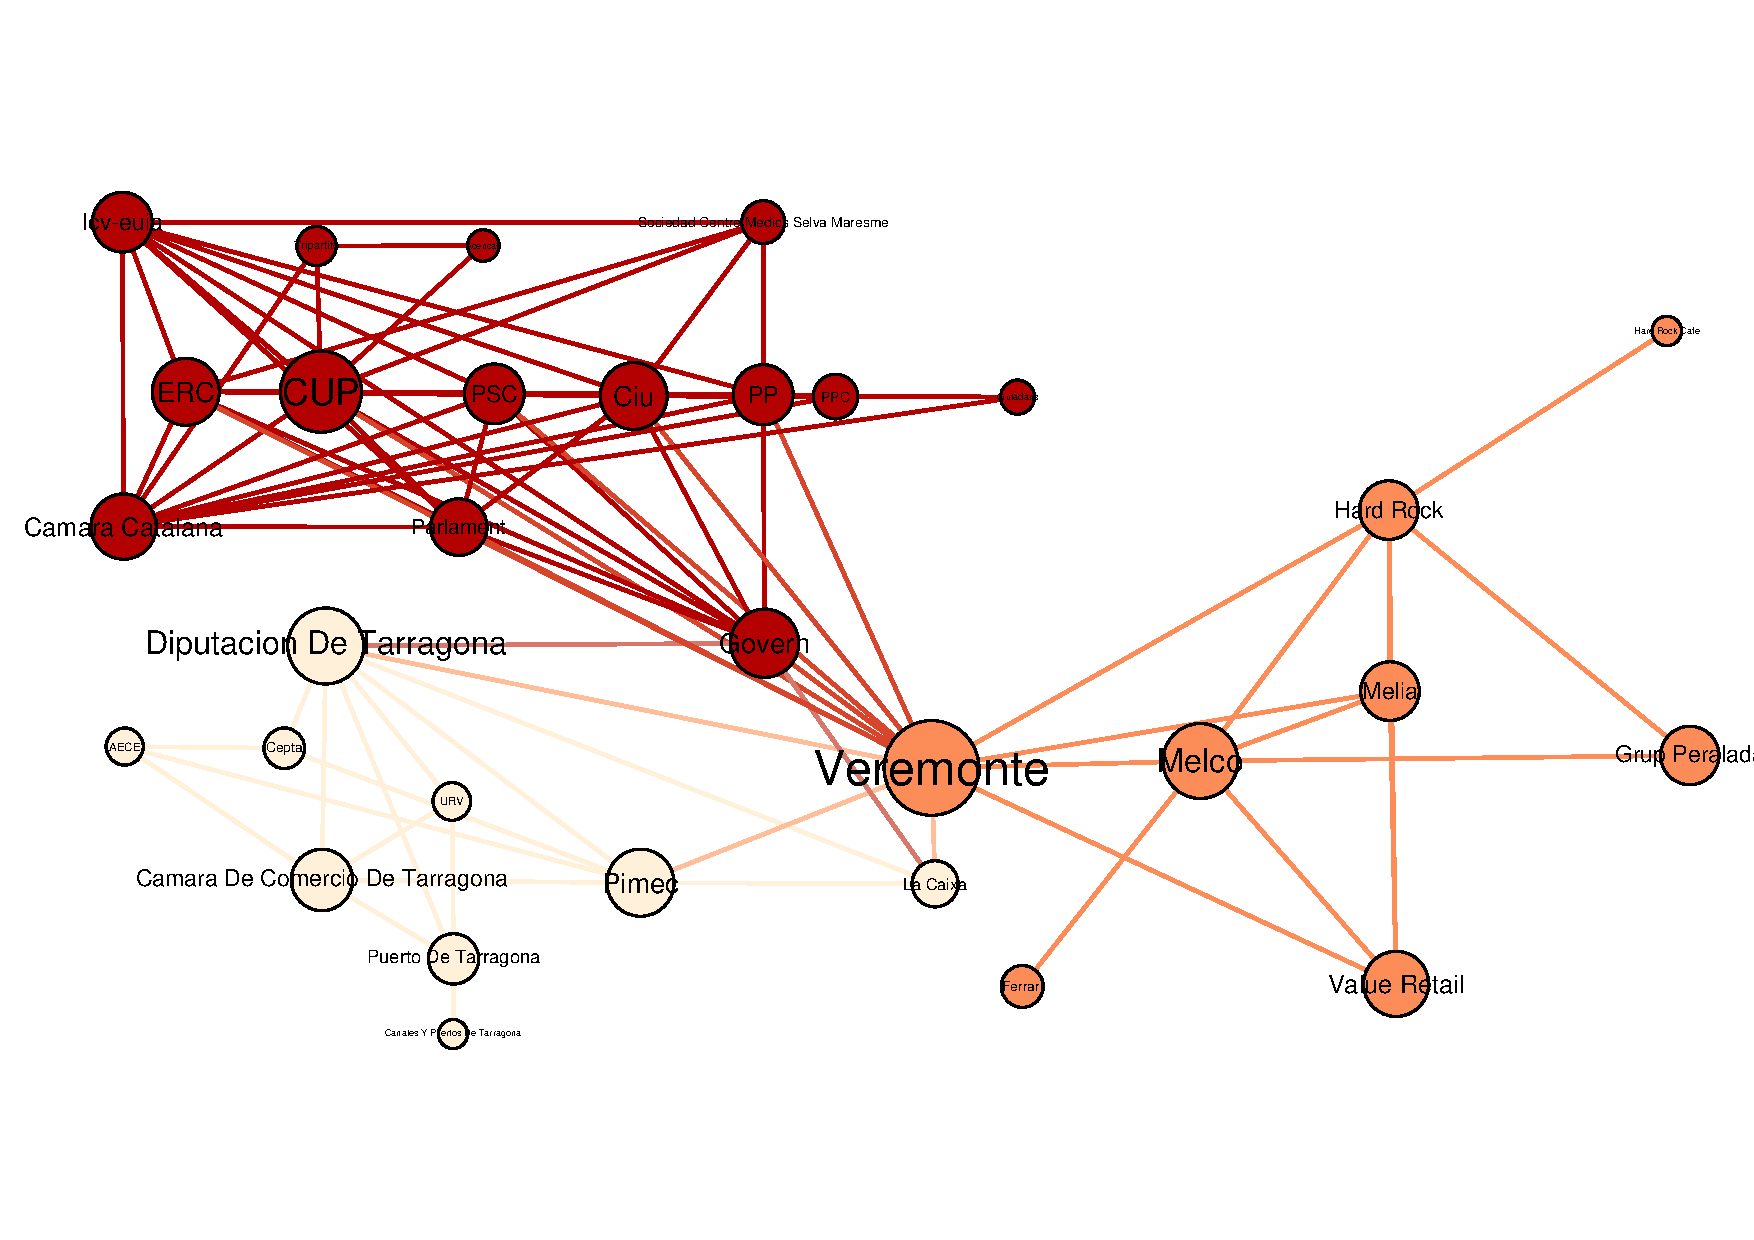
\includegraphics[width=0.9\textwidth]{figs/00062014-organizations}
    \caption{Organizations PN of the BCN-World Bill.}
    \label{fig:00062014-organizations}
\end{figure}


\subsubsection{Person-Organization PN}\label{subsec:bcn_world-person-organization}

Figure \ref{fig:00062014-organizations} shows the PN relating the relationships between the most important persons and organizations related to BCN-World. This graph was constructed by considering all possible relationships between persons and organizations, selecting the most influential persons and organizations as measured by their pagerank and filtering out every node that is not relevant or directly connected to a relevant node. Once more, we show only the giant component due to space constraints.\\

\begin{figure}[H]
    \centering
    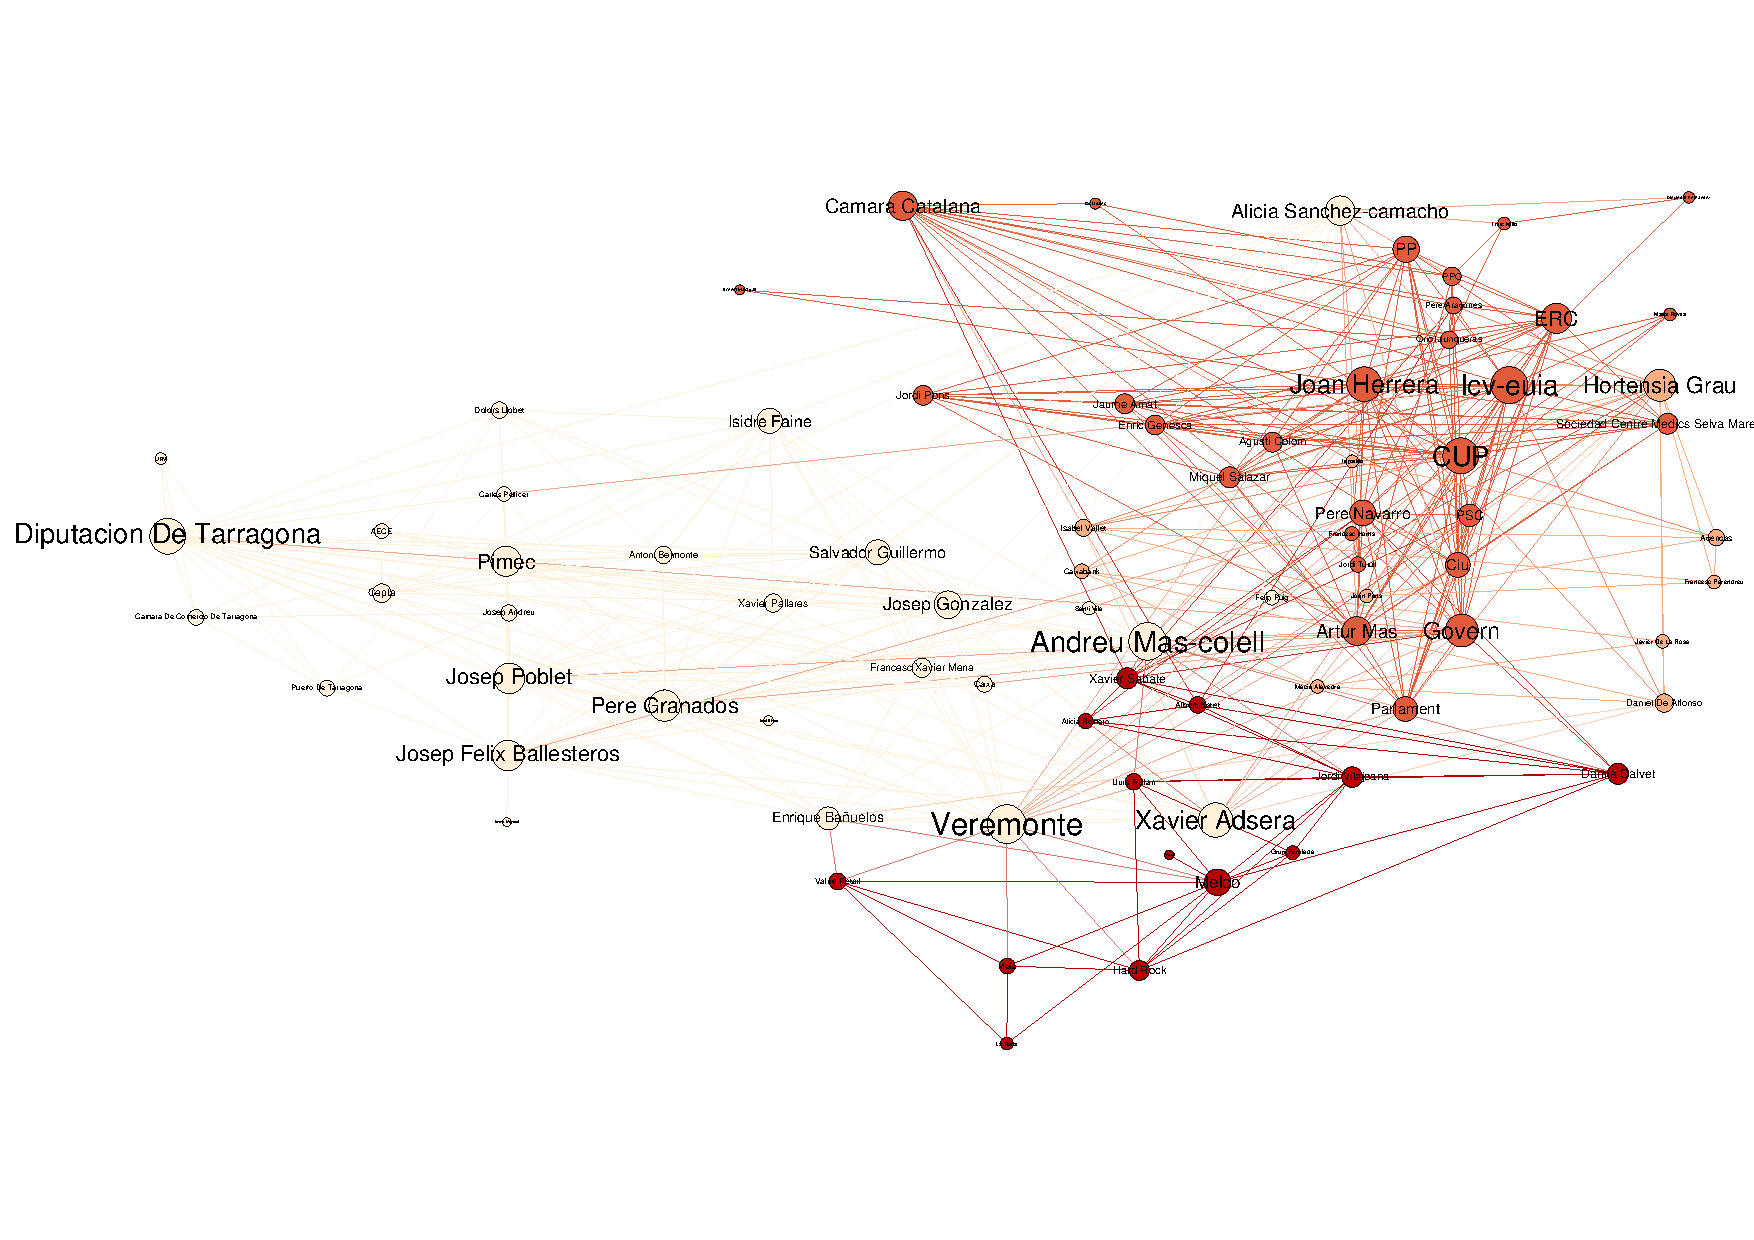
\includegraphics[width=0.9\textwidth]{figs/00062014-person_organizations}
    \caption{Person-Organization PN of the BCN-World Bill.}
    \label{fig:00062014-organizations}
\end{figure}


This graph is bigger in number of nodes but is similar to the Organization-Organization PN. To start with, it features three communities which are related to the communities previously found: a community formed by investors (in the lower right corner), a community of politicians and their political parties (in the upper right corner) and a community of organizations and people related to Tarragona (in the left side). \\
Note that the most relevant actors from the Organization-Organization PN retain their importance: Veremonte, Diputaci\'o de Tarragona, CUP and the Government are highly central. Cambra Catalana (The Catalan Chamber of Commerce) is now slightly more important, as it has many connections with politicians. \\

When it comes to analyzing the role of persons, there are many interesting insights to be gained. First, the most relevant people are Andreu Mas-Colell, the Advisor of Economy and Knowledge of the Catalan Government, and Xavier Adsera, a senior advisor to Veremonte and the president of the BCN-World group. Other relevant entities include Josep Felix Ballesteros, Pere Granados and Josep Poblet, three PSC and CiU mayors of the main towns in Tarragona; Joan Herrera and Hortensia Grau the spokesmen of ICV-EUIA, a party against the project; Artur Mas, the president of the Catalan Government;  Alicia S\'anchez-Camacho, spokeswoman of PP, the ruling party in Spain and Isidre Faine and Enrique Ba\~nuelos, presidents of La Caixa and Veremonte. \\

Something which is particularly interesting is how there intermediary role of Veremonte is reinforced in this PN, showing links with most of the nodes in the other two communities and being also connected to them through Xavier Adsera. By inspecting the news articles, we realize that Adsera was the main negotiator for Veremonte and participated in several key meetings, for instance with Ballesteros, Granados and Poblet, to convince the PSC to vote in favor of the law. \\

An Organization-Person-Person-Organization graph pattern like this might be particularly interesting for detecting lobbying relationships. We find for instance that Veremonte is directly conected to the Catalan Government; these are two organizations that are in turn related to Adsera and Artur Mas who are brokers in charge of connecting their respective organizations. \\

Besides from these interesting insights, this graph also shows some shortcomings of our method. First, there is a giant community made of politicians which does not seem to exhibit any kind of internal sub-structure. Almost all of the politicians of the Parliament are connected with every other politician, instead of, for instance, showing only connections among politicians of the same party. \\

A second shortcoming of this graph is that it fails to detect some relationships which are very important. For instance none of the previously mentioned mayors are related to their political party, something which is particularly important to establish their role as negotiators. This might be because they are mostly referred in the news as mayors of important cities of Tarragona (note how they are strongly linked to most of the institutions of the Tarragona community) instead of being related to their political parties. 


\subsection{Law of Popular Non-referendary Consults}\label{subsec:lpnc}

The Law of Popular Non-referendary Consults (hereinafter LPNC) is a law which was approved in September 2014 to allow the Catalan Government to call for non binding electoral consults to catalan citizens. This law was particularly controversial as it was approved with the main objective of making a consult regarding Catalonia'secession from Spain. Shortly after its approval, Artur Mas, president of the Catalan Government, called for such a consultation to take place on November 9th. The Spanish Government immediately declared its unconstitutionality, which the Supreme Court of Spain availed. \\

The LPNC is particularly interesting because although its a law regulating any type of consultation on public affairs, its controversy lies on its use for the November 9th election. The affected parties are consequently mainly politicians and organizations which are in favor or against Catalan independence.\\

\subsection{Organization PN}\label{subsec:lpnc-organization-organization}

Figure \ref{fig:00062014-organizations} shows the Organization PN for the LPNC. As previously, colors identify communities and font and node size identify importance as measured by the Pagerank of the node. We show only the giant component of the graph.\\


The first relevant observation is that the entities shown in this graph are mostly political parties and NGOs related to the independence of Catalonia. Modularity Clustering yields three communities, shown in the upper left, upper right and bottom sections of the graph. The two communities in the the upper right section are made on the one hand by parties of Spain, Catalonia and other regions of Spain which have independentist claims and, on the other hand, institutions that were involved in determining its constitutionality: the Spanish Senate and House of Representatives (\emph{Senado} and \emph{Congreso}), the Catalan Parliament(\emph{Parlament}) and the Constitutional Court of Spain (\emph{Tribunal Constitucional}). The single community in the bottom of the graph mostly shows pro-independence groups: \emph{Barcelona Decideix}, \emph{Reagrupament}, \emph{Solidaritat} and \emph{Moviment Arenyenc}. \\


\begin{figure}[H]
    \centering
    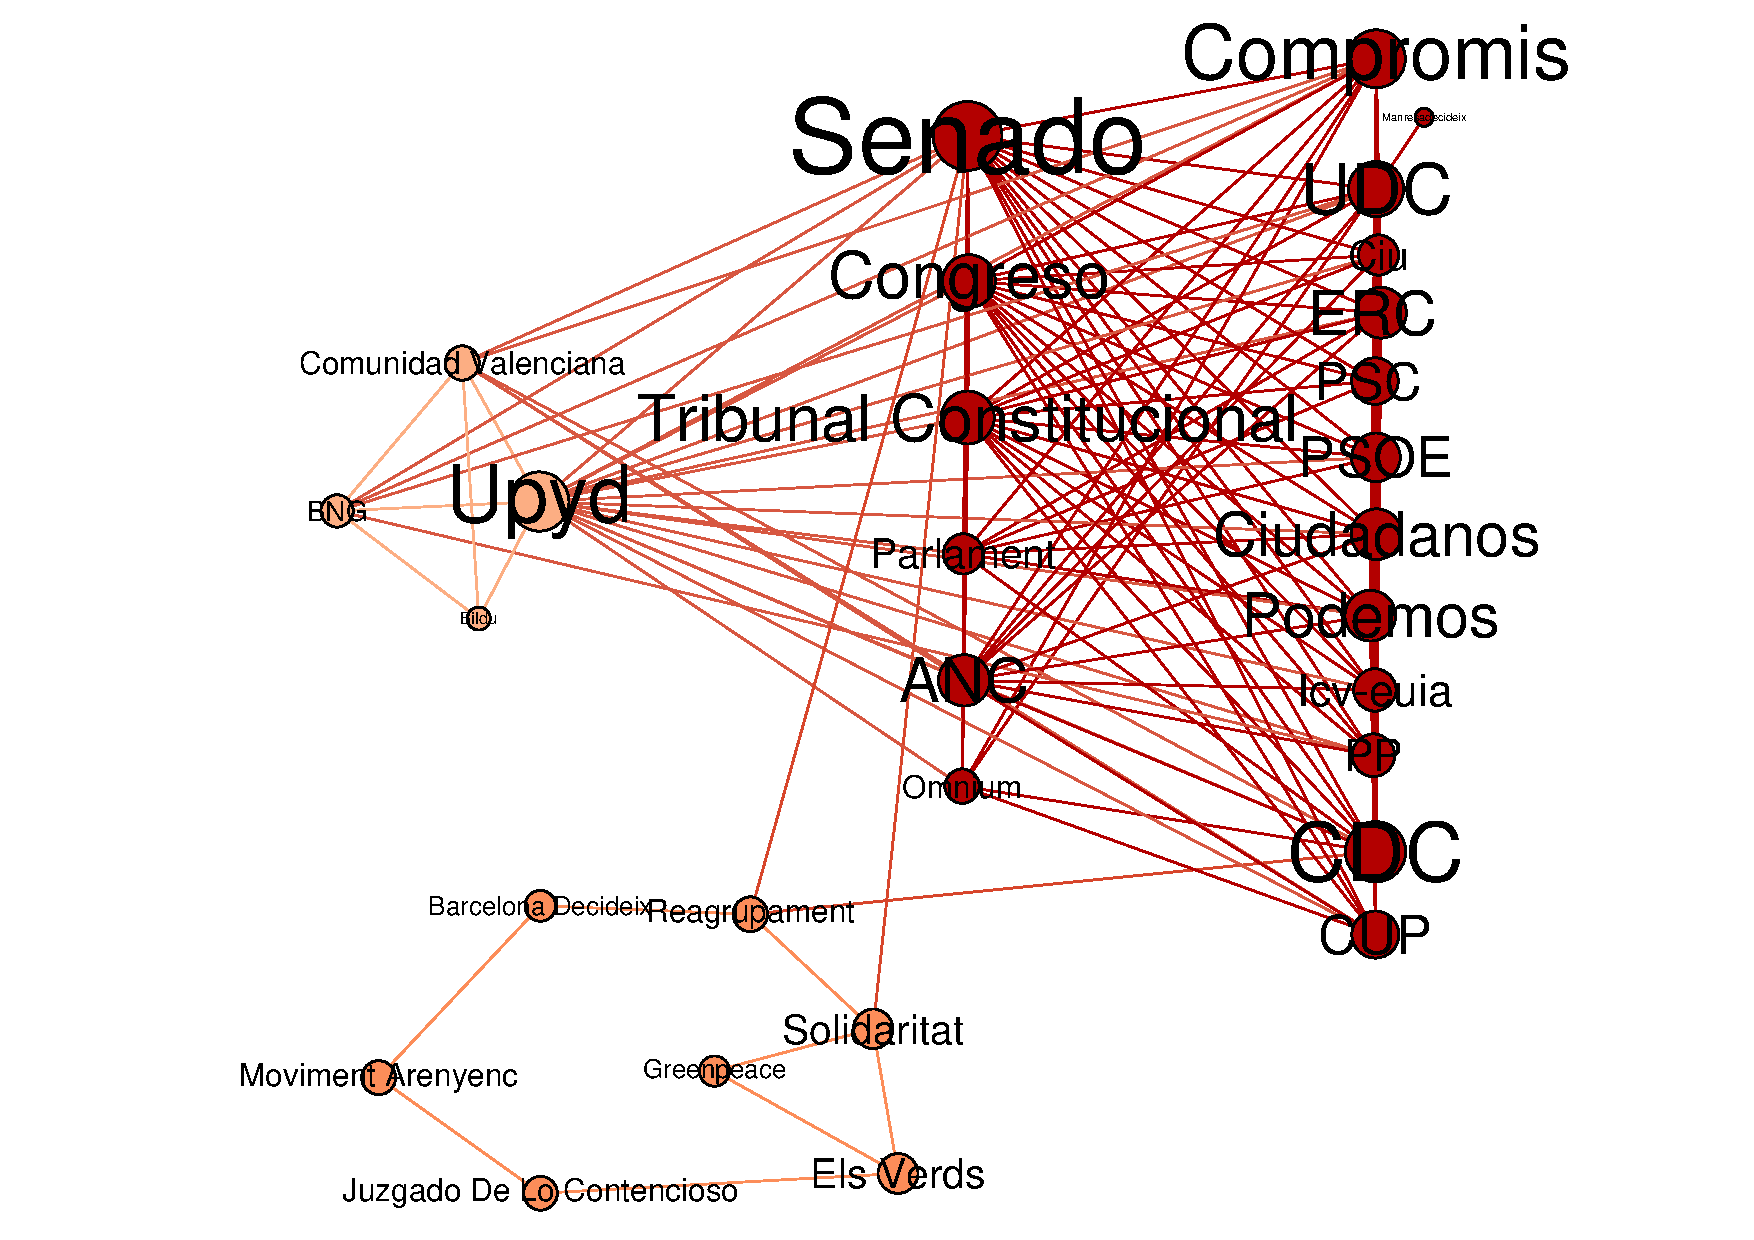
\includegraphics[width=0.9\textwidth]{figs/00102014-organizations}
    \caption{Organization PN for the LPNC bill}
    \label{fig:00102014-organizations}
\end{figure}


Broadly speaking, these communities correctly identify the two types of organizations that are involved with the law, with some exceptions: \emph{ANC} (Assemblea Nacional Catalana, in English National Catalan Assembly) and \emph{Omnium} are NGOs which rather than being connected with the rest of the NGOs are connected with other political parties. This might seem counter-intuitive at first, but if may be because they work more with political parties than with the rest of NGOs. Similarly \emph{Juzgado de lo Contencioso} (Litigation Court) would intuitevely be related with the rest of the political institutions. Finally, note how \emph{Greenpeace} and \emph{Els Verds}, despite not being related, are present in the graph. These might be due to the fact they are too Non-Governmental Organizations, devoted though to environmentalist causes. 

When it comes to assessing the importance of organizations, we find that almost all the political parties, with the exceptions of parties from other regions of Spain, are equally relevant as measured by Pagerank. Also note the importance of the Spanish Senate and Congress, the Catalan Parliament and the Constitutional Court. Among the pro-Independence NGOs, \emph{ANC} is the most preeminent.

\subsection{Person PN}\label{subsec:lpnc-person-organization}

Figure \ref{fig:00102014-persons} shows the Person PN for the LPNC. When analyzing the community structure of the PN, we see that there are seven communities, identified with different colours. In the case of this PN its hard to make sense of the clusters of people identified by modularity clustering. Politicians of different parties and of different regions or instutions, are spread around the graph. \\

On the other hand, looking at individual, widely known politicians, it is possible to make sense of the relations we see. For instance, Mariano Rajoy, the prime minister of Spain, is connected to senior members of PP, his political party, and of other relevant parties. Similarly, senior pro-independence politicians like Artur Mas, Oriol Junqueras, Josep Antoni Duran tend to be connected together. \\

\begin{figure}[H]
    \centering
    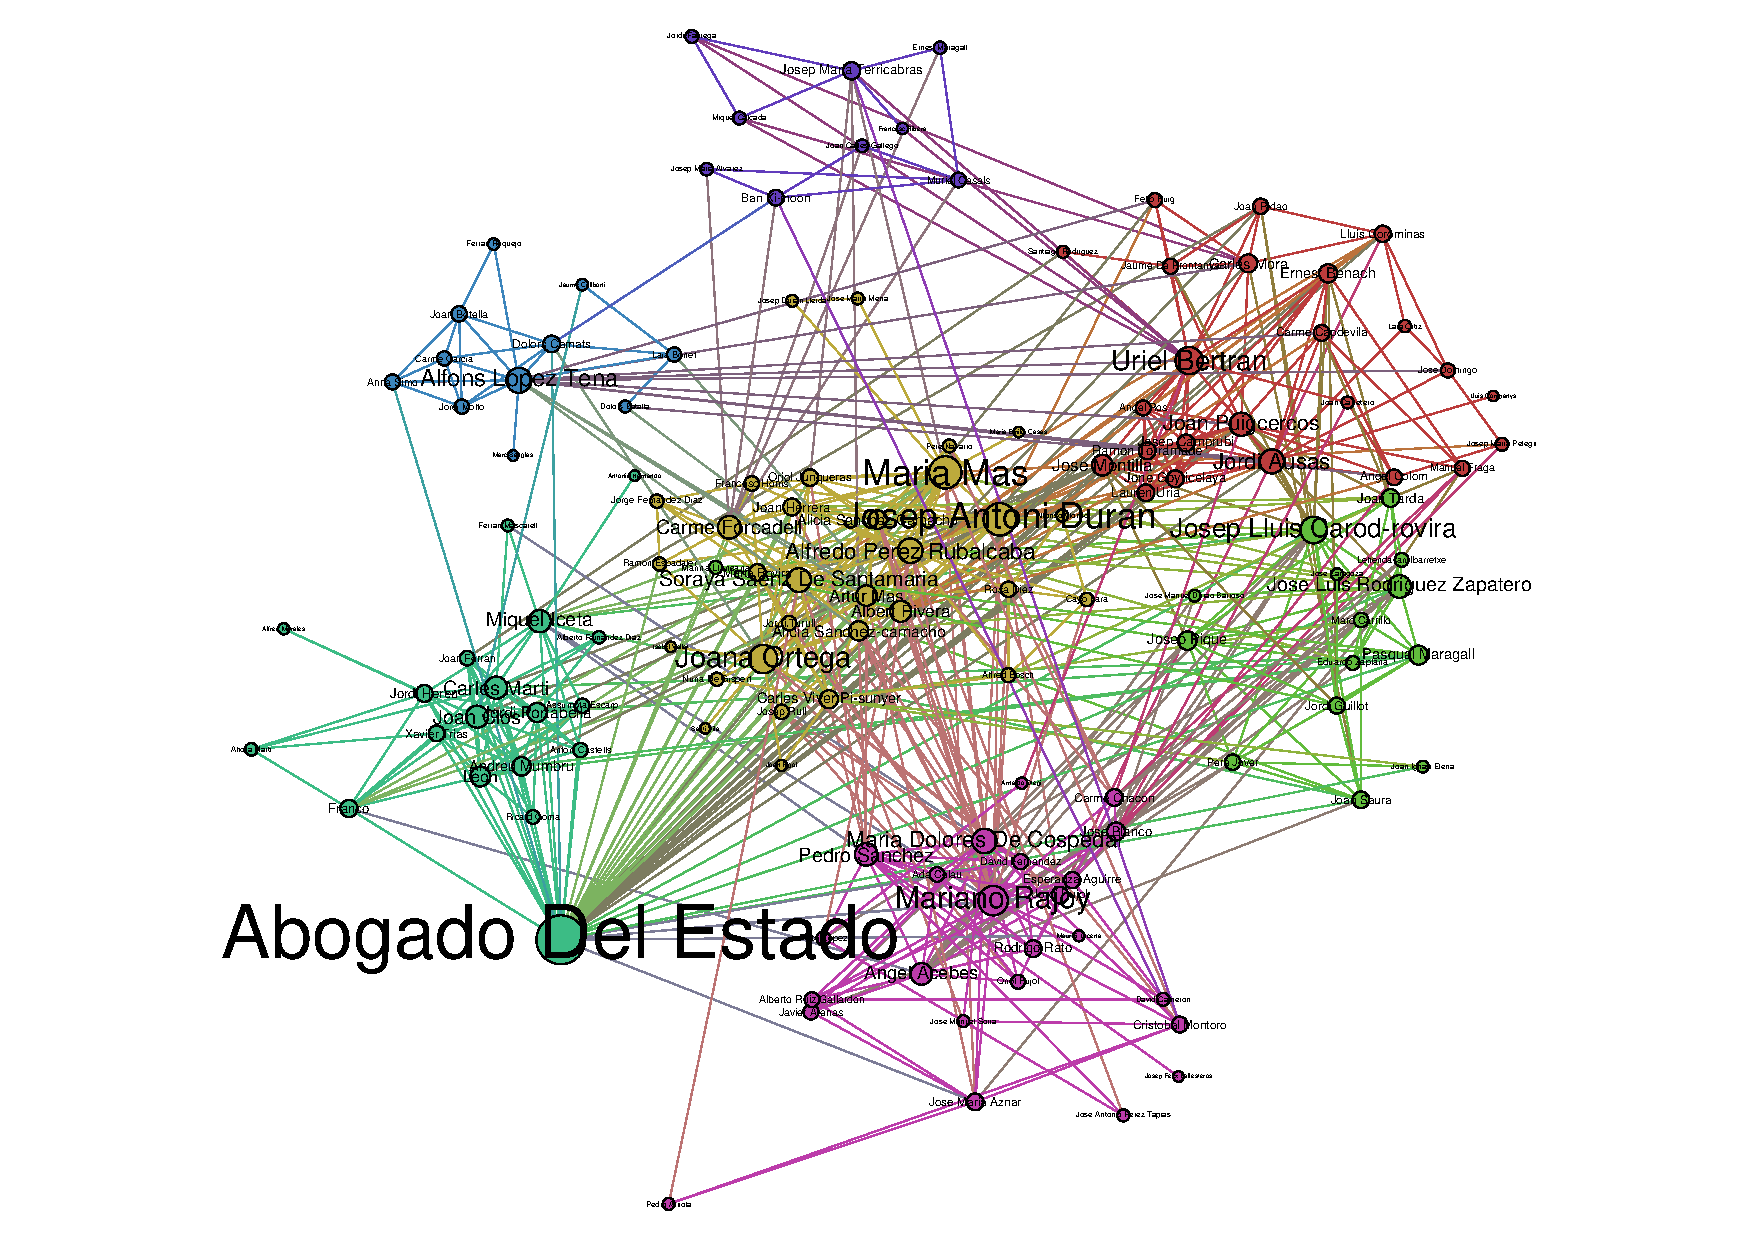
\includegraphics[width=1\textwidth,scale=1.3]{figs/00102014-persons}
    \caption{Person PN for the LPNC bill}
    \label{fig:00102014-persons}
\end{figure}




\newpage
\section{Conclusions}\label{sec:conclusions}

Conclusions come here.

\newpage

\references

 
\appendixECD


\end{document}

